\documentclass[journal,12pt,twocolumn]{IEEEtran}
\usepackage[utf8]{inputenc}
\usepackage{amsmath}
\usepackage{amssymb}
\usepackage{listings}
\usepackage{physics}
\usepackage{tikz}
\newcommand{\myvec}[1]{\ensuremath{\begin{pmatrix}#1\end{pmatrix}}}
\let\vec\mathbf
\usepackage{graphicx}
\graphicspath{ {./images/} }
\newcommand*\mycirc[1]{%
   \begin{tikzpicture}
     \node[draw,circle,inner sep=1pt,color=black ] {#1};
   \end{tikzpicture}}
   
\title{Assignment 3
\\Linear Programming }
\author{Swati Mohanty (EE20RESCH11007) }
\date{October 2020}

\begin{document}

\maketitle


\section{Problem}
Minimise and Maximise $Z=x+2y$ subject to $x+2y\geq100$; $2x-y\leq0$; $2x+y\leq200$; $x,y\leq0$.
\section{Solution}
In order to obtain the maximum and minimum value we need to solve the system of inequalities by adding slack variables. The equations now become:
\begin{align}
    x + 2y - Z =0
    \\
    x + 2y - S_1 = 100
    \\
    2x - y + S_2 = 0
    \\
    2x + y + S_3 = 200
\end{align}
The simplex table can be formed as
\begin{align}
    \myvec{x & y & s_1 & s_2 & s_3 & b \\\hline
    1 & $2$ & -1 & 0 & 0 & 50 \\
    2 & -1 & 0 & 1 & 0 & 0 \\
    2 & 1 & 0 & 0 & 1 & 200 \\\hline
    1 & 2 & 0 & 0 & 0 & 0}
\end{align}
The pivot element is 2 as the minimum ratio 50 occurs for y as the entering variable. Now reducing the simplex matrix we get
\begin{align}
    \myvec{x & y & s_1 & s_2 & s_3 & b \\\hline
    \frac{1}{2} & 1 & \frac{-1}{2} & 0 & 0 & 50 \\
    \frac{5}{2} & 0 & \frac{-1}{2} & 1 & 0 & 50 \\
    \frac{3}{2} & 0 & \frac{1}{2} & 0 & 1 & 150 \\\hline
    1 & 2 & 0 & 0 & 0 & 0}
\end{align}
This can be expressed in the form of matrix inequality for maximization and minimization respectively as:
\begin{align}
    \max_{\{x\}}\vec{c}^T\Vec{x}\\
    s.t \quad \Vec{A}\vec{x}\leq \vec{b} ; \Vec{x} \geq 0
    \\\min_{\{x\}}\vec{c}^T\Vec{x}\\
    s.t \quad \Vec{A}\vec{x}\geq \vec{b} ; \Vec{x} \geq 0
\end{align}
where
\begin{align}
    \Vec{c}=\myvec{1\\2}\\
    \Vec{A}=\myvec{1 & 2\\2 & -1\\2 & 1}\\
    \Vec{b}=\myvec{100\\0\\200}
\end{align}
Solving for Z by this reduction method we get
\begin{align}
    Max Z = 400 
    \\Min Z = 100
\end{align}
This can be solved in Python which generates the result as below: 
\\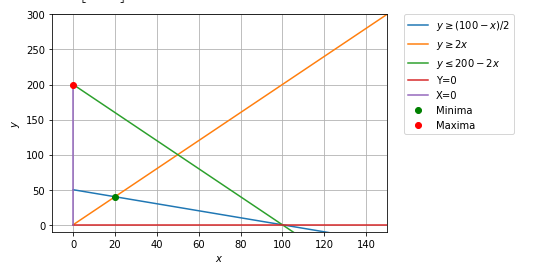
\includegraphics[width=10cm, height=5cm]{plot.jpg}
The following python code generates the maxima and minima values
\\Link : https://github.com/Swati-Mohanty/EE5600/blob/master/Assignment%203/codes/lpp.py
\end{document}